\subsection{Forward Step Problem}

\Figref{forward_step} shows a typical \emph{benchmark} problem in Computational Fluid Dynamics (CFD). It consists of a 2D duct with an inlet (at left) and an outlet of fluid (at right). On the inlet a Couette profile is present due a relative movement between the surfaces. The lower surface speed is set as been $U_0$, while the upper surface speed is set as been null.

 \begin{figure}[h]
 \centering 
 \def\svgwidth{\textwidth}	
\input{figs/forward_step_scheme.pdf_tex}\caption{Forward step problem with a linear inlet velocity profile.}\label{fig:forward_step}
\end{figure}

The analytic solution of Reynolds Equation on the stationary state (there is no squeeze flow) is calculated making the right hand side of \eqref{reynoldseq} equal to zero and integrating it. This way the fluid flux is obtained on the inlet $Q_{in}$ been equal to:
\begin{equation*}
Q_{in}=-\left.\frac{H^3}{12\mu}\frac{\partial p}{\partial x}\right|_l+\frac{U_0}{2}H
.
\end{equation*}
This calculation is repeated for the fluid flux on the outlet $Q_{out}$, this time replacing $H$ by $H/2$ so the Couette flow on the outlet will be half the Couette flow on the input. As $Q_{in}=Q_{out}$ must be accomplish, a Poiuseille flow must appear on the outflow, which is the same, a negative pressure gradient is generated in order to compensate the lack on the Couette term. In fact, this gradient can be computed to be:
\begin{equation*}
\left.\frac{\partial p}{\partial x}\right|_{out} = 6\,a\,\mu\frac{(H/2-H)}{(H/2)^3}.\label{eq:pressure_gap}
\end{equation*}

\begin{figure}[h!]\hspace*{-1cm}
\resizebox{17cm}{!}{
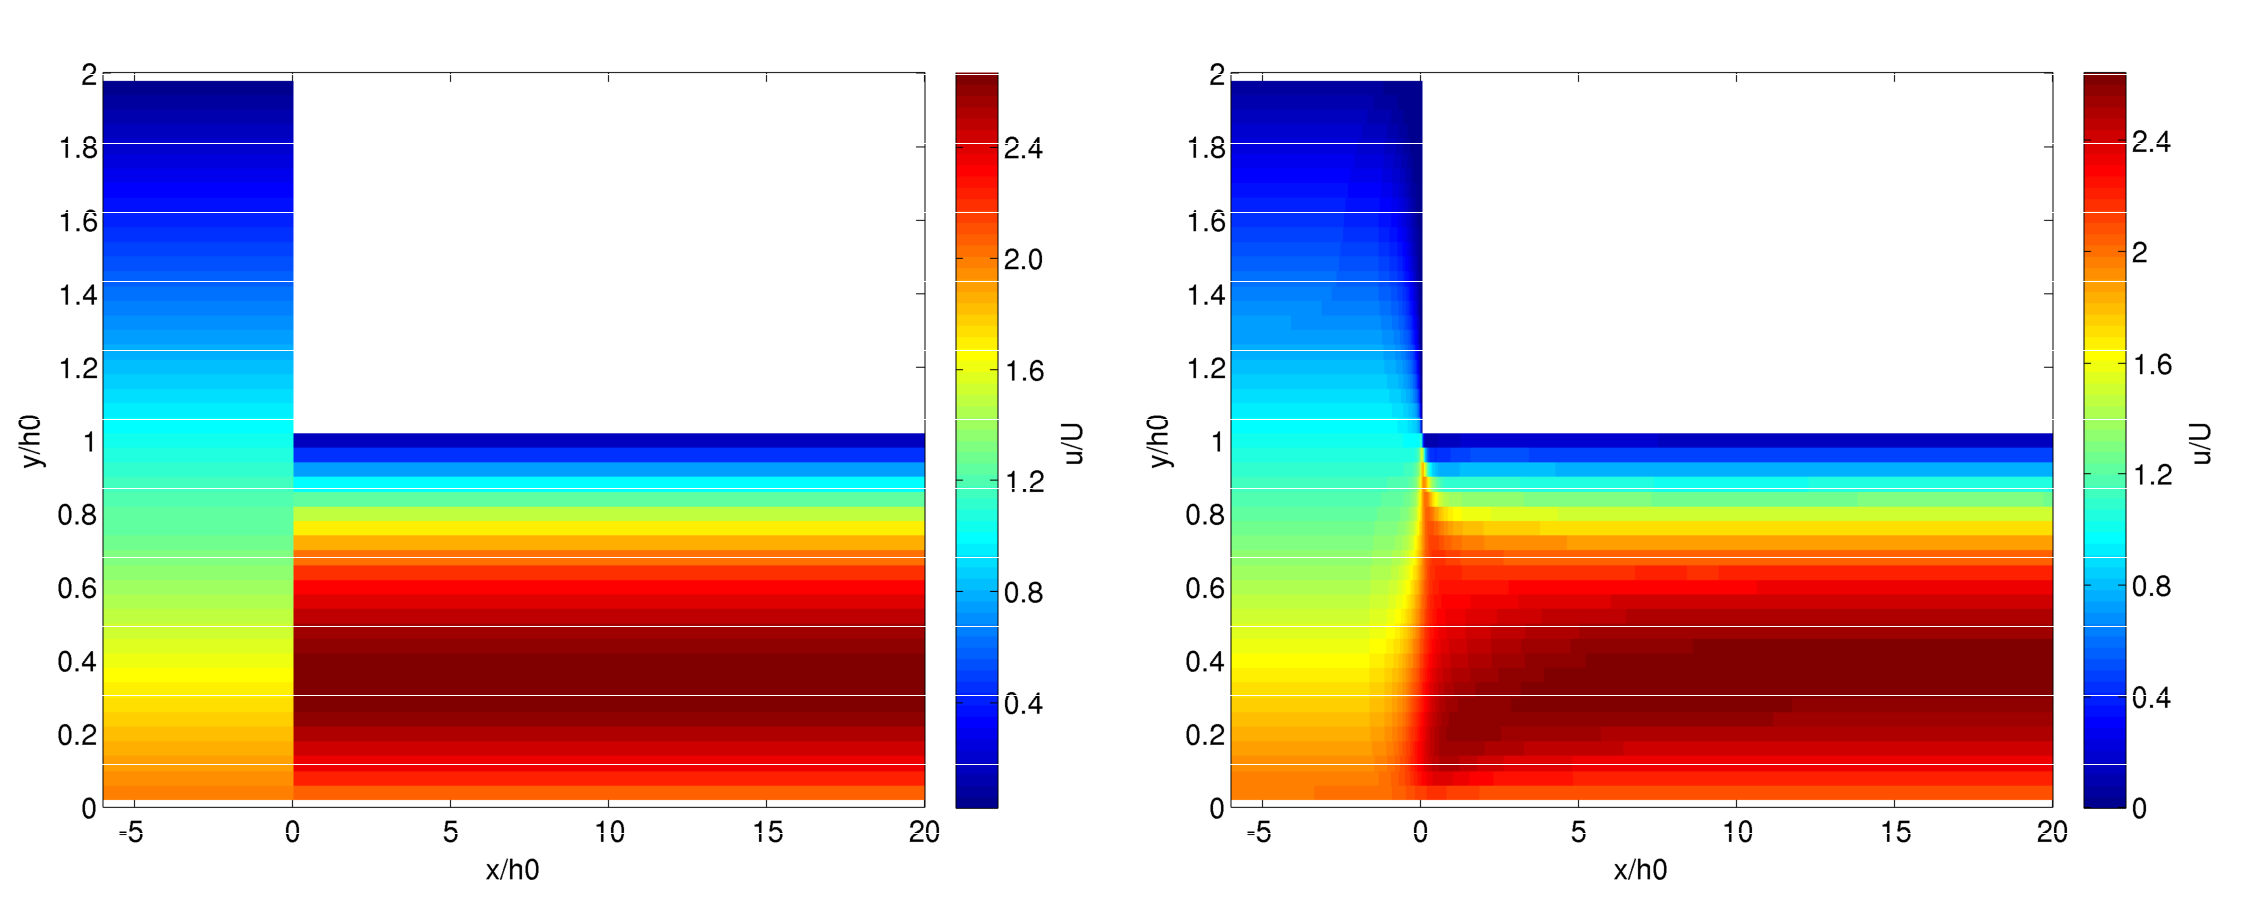
\includegraphics{u_profiles_REQ_NSE.pdf}}
\caption{Horizontal velocity obtained by Reynolds (left fig.) and Navier-Stokes (right fig.) equations for $\text{Re}=100$. $U=U_0/2$, $h_0=H/2$.}\label{fig:u_prof_RE_NS}
\end{figure}

\Figref{u_prof_RE_NS} shows the velocity obtained by both Reynolds and Navier-Stokes equations. Notice the linear profile at the inlet (left side) and the non-linear (parabolic plus linear) on the outlet due to Couette and Poiseuille flows. It can be observed how the field $u$ changes suddenly at $x=0$ for the Reynolds solution. Obviously, this is due to a discontinuity of the gap $h$ there. On the other hand, the Navier-Stokes solution changes softly. In spite of that, they differ only by $1\%$ both in velocities and pressure.